\documentclass[conference]{IEEEtran}
\IEEEoverridecommandlockouts

\usepackage{cite}
\usepackage{amsmath,amssymb,amsfonts}
\usepackage{graphicx}
\usepackage{textcomp}
\usepackage{xcolor}
\usepackage{booktabs}
\usepackage{multirow}
\usepackage{url}

\def\BibTeX{{\rm B\kern-.05em{\sc i\kern-.025em b}\kern-.08em
    T\kern-.1667em\lower.7ex\hbox{E}\kern-.125emX}}

\begin{document}

\title{A Comparative Analysis of BiLSTM and Transformer Architectures for Dynamic Hand Gesture Recognition}

\author{
\IEEEauthorblockN{Marc'Antonio Lopez}
\IEEEauthorblockA{\textit{Polytechnic University of Turin}\\
Turin, Italy\\
marcantoniolopez@polito.it}
\and
\IEEEauthorblockN{Nicole Dalia Cilia}
\IEEEauthorblockA{\textit{University of Enna ``Kore''}\\
Enna, Italy\\
nicoledalia.cilia@unikore.it}
}

\maketitle

\begin{abstract}
This paper presents a rigorous comparative analysis of Bidirectional LSTM (BiLSTM) with Attention and Encoder-only Transformer architectures for dynamic hand gesture recognition using the DYLEM-GRID dataset. We implement a complete PyTorch Lightning-based pipeline with automated hyperparameter optimization via Optuna and systematic ablation studies using 5-fold stratified cross-validation. Our results demonstrate that the BiLSTM model achieves 97.25\% $\pm$ 0.94\% accuracy, outperforming the Transformer (94.75\% $\pm$ 0.94\%). Ablation studies reveal that the attention mechanism is crucial for BiLSTM performance, yielding a 7-percentage-point improvement over models without attention. For Transformers, larger model dimensions (d\_model=128) and max/cls pooling strategies significantly improve accuracy. Both models are trained on data preprocessed through per-class outlier removal and PCA retaining 95\% variance. All code and data are publicly available on HuggingFace Hub.
\end{abstract}

\begin{IEEEkeywords}
Dynamic Hand Gesture Recognition, Deep Learning, BiLSTM, Transformer, Attention Mechanism, Cross-Validation, Ablation Study
\end{IEEEkeywords}

\section{Introduction}

Dynamic Hand Gesture Recognition (D-HGR) is a fundamental task in Human-Computer Interaction (HCI), requiring the modeling of complex spatial and temporal dependencies in sequential motion data. While traditional methods such as Hidden Markov Models (HMMs) \cite{rabiner1989} and Dynamic Time Warping have been employed, deep learning approaches have demonstrated superior performance for sequential data analysis.

Recurrent Neural Networks (RNNs), particularly Long Short-Term Memory (LSTM) \cite{hochreiter1997} networks, became the standard for sequential tasks due to their ability to maintain internal state and mitigate the vanishing gradient problem. The addition of attention mechanisms \cite{bahdanau2014} further enhanced RNNs by enabling adaptive focus on the most relevant time steps. More recently, Transformer architectures \cite{vaswani2017} have achieved state-of-the-art results across multiple domains by using self-attention to model global dependencies without recurrence.

This paper contributes a rigorous, reproducible benchmark comparing these two leading architectures on the DYLEM-GRID dataset \cite{dylem2024}. Our key contributions are:

\begin{itemize}
    \item A modular PyTorch Lightning implementation with HuggingFace Hub integration for reproducibility.
    \item Systematic hyperparameter optimization using Optuna with cross-validation.
    \item Comprehensive ablation studies quantifying the impact of architectural choices.
    \item Empirical evidence that attention mechanisms provide critical performance gains for BiLSTM models on skeletal gesture data.
\end{itemize}

\section{Related Work}

\subsection{Traditional Methods}
Early approaches to gesture recognition relied heavily on template-matching techniques. Dynamic Time Warping (DTW) was widely adopted for its ability to align temporal sequences of varying lengths, making it suitable for gestures performed at different speeds. Hidden Markov Models (HMMs) \cite{rabiner1989} provided a probabilistic framework for modeling the sequential nature of gestures, representing each gesture as a sequence of hidden states with observable emissions. While these methods proved effective in controlled laboratory scenarios with limited gesture vocabularies, they suffer from significant limitations: extensive manual feature engineering is required to extract discriminative representations from raw sensor data, and their performance degrades substantially when confronted with high-dimensional feature spaces or increased gesture complexity. Additionally, these traditional approaches often struggle to generalize across different users or environmental conditions without extensive recalibration.

\subsection{Deep Learning Approaches}
The advent of deep learning revolutionized sequential data processing. Recurrent Neural Networks (RNNs) enabled end-to-end learning directly from raw or minimally processed data, eliminating the need for handcrafted features. However, vanilla RNNs suffered from the vanishing gradient problem, limiting their ability to capture long-range temporal dependencies. Long Short-Term Memory (LSTM) networks \cite{hochreiter1997} addressed this limitation through a gating mechanism that controls information flow, allowing the network to selectively remember or forget information over extended time horizons. Bidirectional variants (BiLSTMs) further enhanced temporal modeling by processing sequences in both forward and backward directions, enabling the model to leverage both past and future context when making predictions at each time step.

Attention mechanisms \cite{bahdanau2014} represented another significant advancement, allowing models to dynamically focus on the most relevant portions of the input sequence rather than relying solely on fixed-length hidden state representations. This proved particularly valuable for gesture recognition, where discriminative information may be concentrated in specific temporal segments (e.g., the peak of a waving motion or the crossing point in air quotes).

More recently, the Transformer architecture \cite{vaswani2017} eliminated recurrence entirely in favor of self-attention mechanisms that compute pairwise relationships between all time steps simultaneously. This approach offers several advantages: parallel computation enables efficient training on modern hardware, and the attention mechanism can directly model long-range dependencies without the information bottleneck inherent in recurrent architectures. While Transformers have achieved remarkable success in natural language processing and are increasingly applied to time-series classification \cite{zerveas2021}, their effectiveness for gesture recognition---particularly on smaller datasets---remains an active area of investigation. Our work contributes empirical evidence on the relative strengths of these architectures for skeletal gesture data.

\section{Dataset and Methodology}

\subsection{The DYLEM-GRID Dataset}
We utilize the DYLEM-GRID (Dynamic Leap Motion Gesture Recognition Indexed Dataset) \cite{dylem2024}, a purpose-built corpus for evaluating deep learning approaches to dynamic hand gesture recognition. The dataset is publicly available on Kaggle and the accompanying codebase on GitHub, ensuring full reproducibility of our experiments.

\subsubsection{Data Acquisition}
The dataset was captured using an Ultraleap Leap Motion Controller 2, a near-infrared optical sensor employing two infrared cameras and three LEDs to track hand movements with sub-millimeter precision. Data was recorded at a sampling frequency of approximately 30 Hz. Participants were instructed to stand at a fixed distance from the sensor and position their palms approximately 40 cm above the device to ensure consistency across recordings.

\subsubsection{Gesture Vocabulary}
The dataset comprises 400 recordings of four semantically distinct dynamic hand gestures. The gestures were collected from multiple participants, with each participant performing all four gesture types. The gestures were selected for their cross-linguistic universality and prevalence in natural human-computer interaction:

\begin{itemize}
    \item \textbf{Air Quotes}: Both hands are raised to shoulder height with index and middle fingers extended. The user flexes these fingers in a downward motion to simulate quotation marks---a gesture commonly used to indicate irony or skepticism.
    
    \item \textbf{Finger Wagging}: One arm is extended forward with the index finger pointing upward. The finger moves side-to-side in a rhythmic motion, commonly used as an admonishing or warning gesture.
    
    \item \textbf{Waving}: One arm is extended with the hand open and facing forward. The hand moves side-to-side in a continuous arc, rotating at the wrist---a universal greeting gesture.
    
    \item \textbf{Zoom}: One hand is held with thumb and index finger pinched together. The user moves these fingers apart to ``zoom in'' or closer together to ``zoom out''---a gesture popularized by touchscreen interfaces.
\end{itemize}

\subsubsection{Feature Representation}
Each time step captures 244 distinct features representing the positional and rotational data of 27 unique hand elements (palm, wrist, and 25 finger bones/joints). These features comprehensively encode palm position, orientation, velocity, and the position, direction, and width of each finger bone, enabling detailed kinematic analysis of hand movements across the entire gesture trajectory.

\subsubsection{Dataset Versions}
The DYLEM-GRID dataset is provided in three versions to accommodate different research needs:

\begin{enumerate}
    \item \textbf{DYLEM-GRID\_Raw}: Contains unprocessed time-series data with variable sequence lengths and all 244 original features.
    
    \item \textbf{DYLEM-GRID\_Cleaned}: A preprocessed version with redundant features removed (reducing to 174 features), sequence lengths equalized via padding, and values normalized to $[-1, 1]$. This version is optimized for recurrent neural network training.
    
    \item \textbf{DYLEM-GRID\_Statistic}: A time-independent, feature-engineered version where each gesture is represented by 696 statistical features (mean, max, min, and standard deviation of each of the 174 cleaned features). This version supports classical machine learning algorithms.
\end{enumerate}

All versions follow an 80/20 train/test split, with data organized into gesture-specific subdirectories for convenient loading.

\subsection{Preprocessing Pipeline}
Our preprocessing pipeline is implemented as a PyTorch Lightning \texttt{DataModule}, ensuring reproducibility and seamless integration with the training framework. The pipeline addresses several challenges inherent in raw sensor data:

\begin{enumerate}
    \item \textbf{Data Cleaning}: Missing values (NaN) are imputed using backward fill to maintain temporal coherence. Duplicate columns arising from sensor redundancy are removed, and low-variance features (where $>$90\% of values are identical) are eliminated as they provide minimal discriminative information.
    
    \item \textbf{Per-Class Outlier Removal}: Rather than applying global outlier detection, we perform class-specific outlier removal. For each gesture class, values exceeding 3$\sigma$ from the class mean are replaced with the class mean. This approach preserves gesture-specific variations that might otherwise be flagged as outliers when analyzed globally---for example, the extended arm positions in ``waving'' that would appear unusual compared to the compact hand positions in ``zoom''.
    
    \item \textbf{Normalization}: Min-max scaling transforms all features to the $[0, 1]$ range, ensuring that features with larger magnitudes (e.g., palm position in millimeters) do not dominate features with smaller scales (e.g., finger bone directions as unit vectors).
    
    \item \textbf{Class Balancing}: Although the original dataset is balanced, our pipeline includes an oversampling mechanism that duplicates minority class samples to match the majority class count, ensuring robustness to future dataset extensions with imbalanced classes.
    
    \item \textbf{PCA}: Principal Component Analysis reduces dimensionality while retaining 95\% of explained variance, compressing the original 174 post-cleaning features to approximately 24 principal components. This reduction mitigates the curse of dimensionality and accelerates training without significant information loss.
    
    \item \textbf{Padding}: Variable-length sequences are zero-padded to the maximum sequence length in the dataset, enabling efficient batch processing while maintaining temporal structure.
\end{enumerate}

\subsection{Cross-Validation Protocol}
To ensure statistically robust performance estimates, all experiments employ 5-fold stratified cross-validation with a fixed random seed (42) for reproducibility. Stratification guarantees that each fold maintains the same class distribution as the full dataset, preventing sampling bias that could inflate or deflate accuracy estimates. Each model configuration is trained and evaluated independently on all five folds, and we report the mean accuracy $\pm$ standard deviation across folds. This protocol provides both a central tendency estimate and a measure of variance, enabling meaningful comparison between architectures even when differences are modest.

\section{Model Architectures}

\subsection{BiLSTM with Attention (GestureRNN)}
Our BiLSTM architecture is designed to capture bidirectional temporal dependencies while enabling selective focus on discriminative time steps through an attention mechanism. The model first processes the input sequence through a multi-layer bidirectional LSTM, producing hidden states that encode both past and future context at each time step. For a sequence of length $T$, the BiLSTM produces hidden states $\mathbf{h}_t \in \mathbb{R}^{2H}$ (where $H$ is the hidden dimension) by concatenating the forward and backward LSTM outputs.

Rather than relying solely on the final hidden state---which may inadequately summarize long sequences---we apply an additive attention mechanism:

\begin{equation}
\alpha_t = \text{softmax}(\mathbf{W}_a \mathbf{h}_t)
\end{equation}
\begin{equation}
\mathbf{c} = \sum_{t=1}^{T} \alpha_t \mathbf{h}_t
\end{equation}

\noindent where $\mathbf{W}_a$ is a learned attention weight matrix and $\alpha_t$ represents the attention weight assigned to time step $t$. The resulting context vector $\mathbf{c}$ is a weighted combination of all hidden states, with the model learning to emphasize time steps most relevant for classification. This mechanism is particularly valuable for gesture recognition, where discriminative information may be concentrated in specific motion phases (e.g., the apex of a wave or the crossing point of air quotes).

The context vector is then processed through a classifier consisting of a linear layer, batch normalization for training stability, ReLU activation, dropout for regularization, and a final linear layer producing class logits. This architecture balances expressiveness with regularization, preventing overfitting on the relatively small dataset.

\subsection{Transformer Encoder (GestureTransformer)}
Our Transformer architecture adapts the encoder portion of the original Transformer \cite{vaswani2017} for sequence classification. Unlike the BiLSTM, which processes sequences recurrently, the Transformer relies entirely on self-attention to model temporal relationships, offering potential advantages in capturing long-range dependencies and enabling parallelized training.

The model first projects input features to $d\_model$ dimensions through a linear layer, then adds sinusoidal positional encoding to inject temporal order information that would otherwise be lost due to the permutation-invariant nature of attention:

\begin{equation}
PE_{(pos, 2i)} = \sin(pos / 10000^{2i / d_{model}})
\end{equation}
\begin{equation}
PE_{(pos, 2i+1)} = \cos(pos / 10000^{2i / d_{model}})
\end{equation}

The encoded sequence is processed through $L$ Transformer encoder layers, each containing multi-head self-attention followed by a position-wise feedforward network with GELU activation. Multi-head attention enables the model to attend to different representation subspaces simultaneously, potentially capturing diverse temporal patterns.

Unlike sequence-to-sequence tasks, classification requires aggregating the variable-length encoded sequence into a fixed-length representation. We implement three configurable pooling strategies: \textbf{mean pooling} (averaging all time step representations), \textbf{max pooling} (taking the element-wise maximum), and \textbf{CLS pooling} (prepending a learnable classification token and using its final representation). The pooled representation is then passed through a feedforward classifier to produce class predictions.

\section{Experiments and Results}

\subsection{Hyperparameter Optimization}
We conducted Optuna-based hyperparameter search with 100 trials per model using median pruning. Table~\ref{tab:optuna} summarizes the optimal configurations.

\begin{table}[htbp]
\caption{Optimized Hyperparameters}
\label{tab:optuna}
\centering
\begin{tabular}{lcc}
\toprule
\textbf{Parameter} & \textbf{BiLSTM} & \textbf{Transformer} \\
\midrule
hidden\_size / d\_model & 128 & 128 \\
num\_layers & 2 & 2 \\
nhead & -- & 8 \\
dim\_feedforward & -- & 256 \\
dropout & 0.262 & 0.137 \\
learning\_rate & 3.47e-4 & 2.59e-3 \\
optimizer & Adam & AdamW \\
\bottomrule
\end{tabular}
\end{table}

\subsection{Cross-Validation Results}
Table~\ref{tab:cv_results} presents the 5-fold cross-validation results with optimized hyperparameters.

\begin{table}[htbp]
\caption{5-Fold Cross-Validation Results}
\label{tab:cv_results}
\centering
\begin{tabular}{lccc}
\toprule
\textbf{Model} & \textbf{Accuracy} & \textbf{F1 Score} & \textbf{Avg. Epochs} \\
\midrule
BiLSTM + Attention & \textbf{97.25\% $\pm$ 0.94\%} & 97.26\% & 35.4 \\
Transformer & 94.75\% $\pm$ 0.94\% & 94.78\% & 31.8 \\
\bottomrule
\end{tabular}
\end{table}

The BiLSTM model achieves 2.5 percentage points higher accuracy than the Transformer, suggesting that for this dataset size and task, recurrent architectures with attention may capture the temporal dynamics more effectively.

\begin{figure}[htbp]
\centering
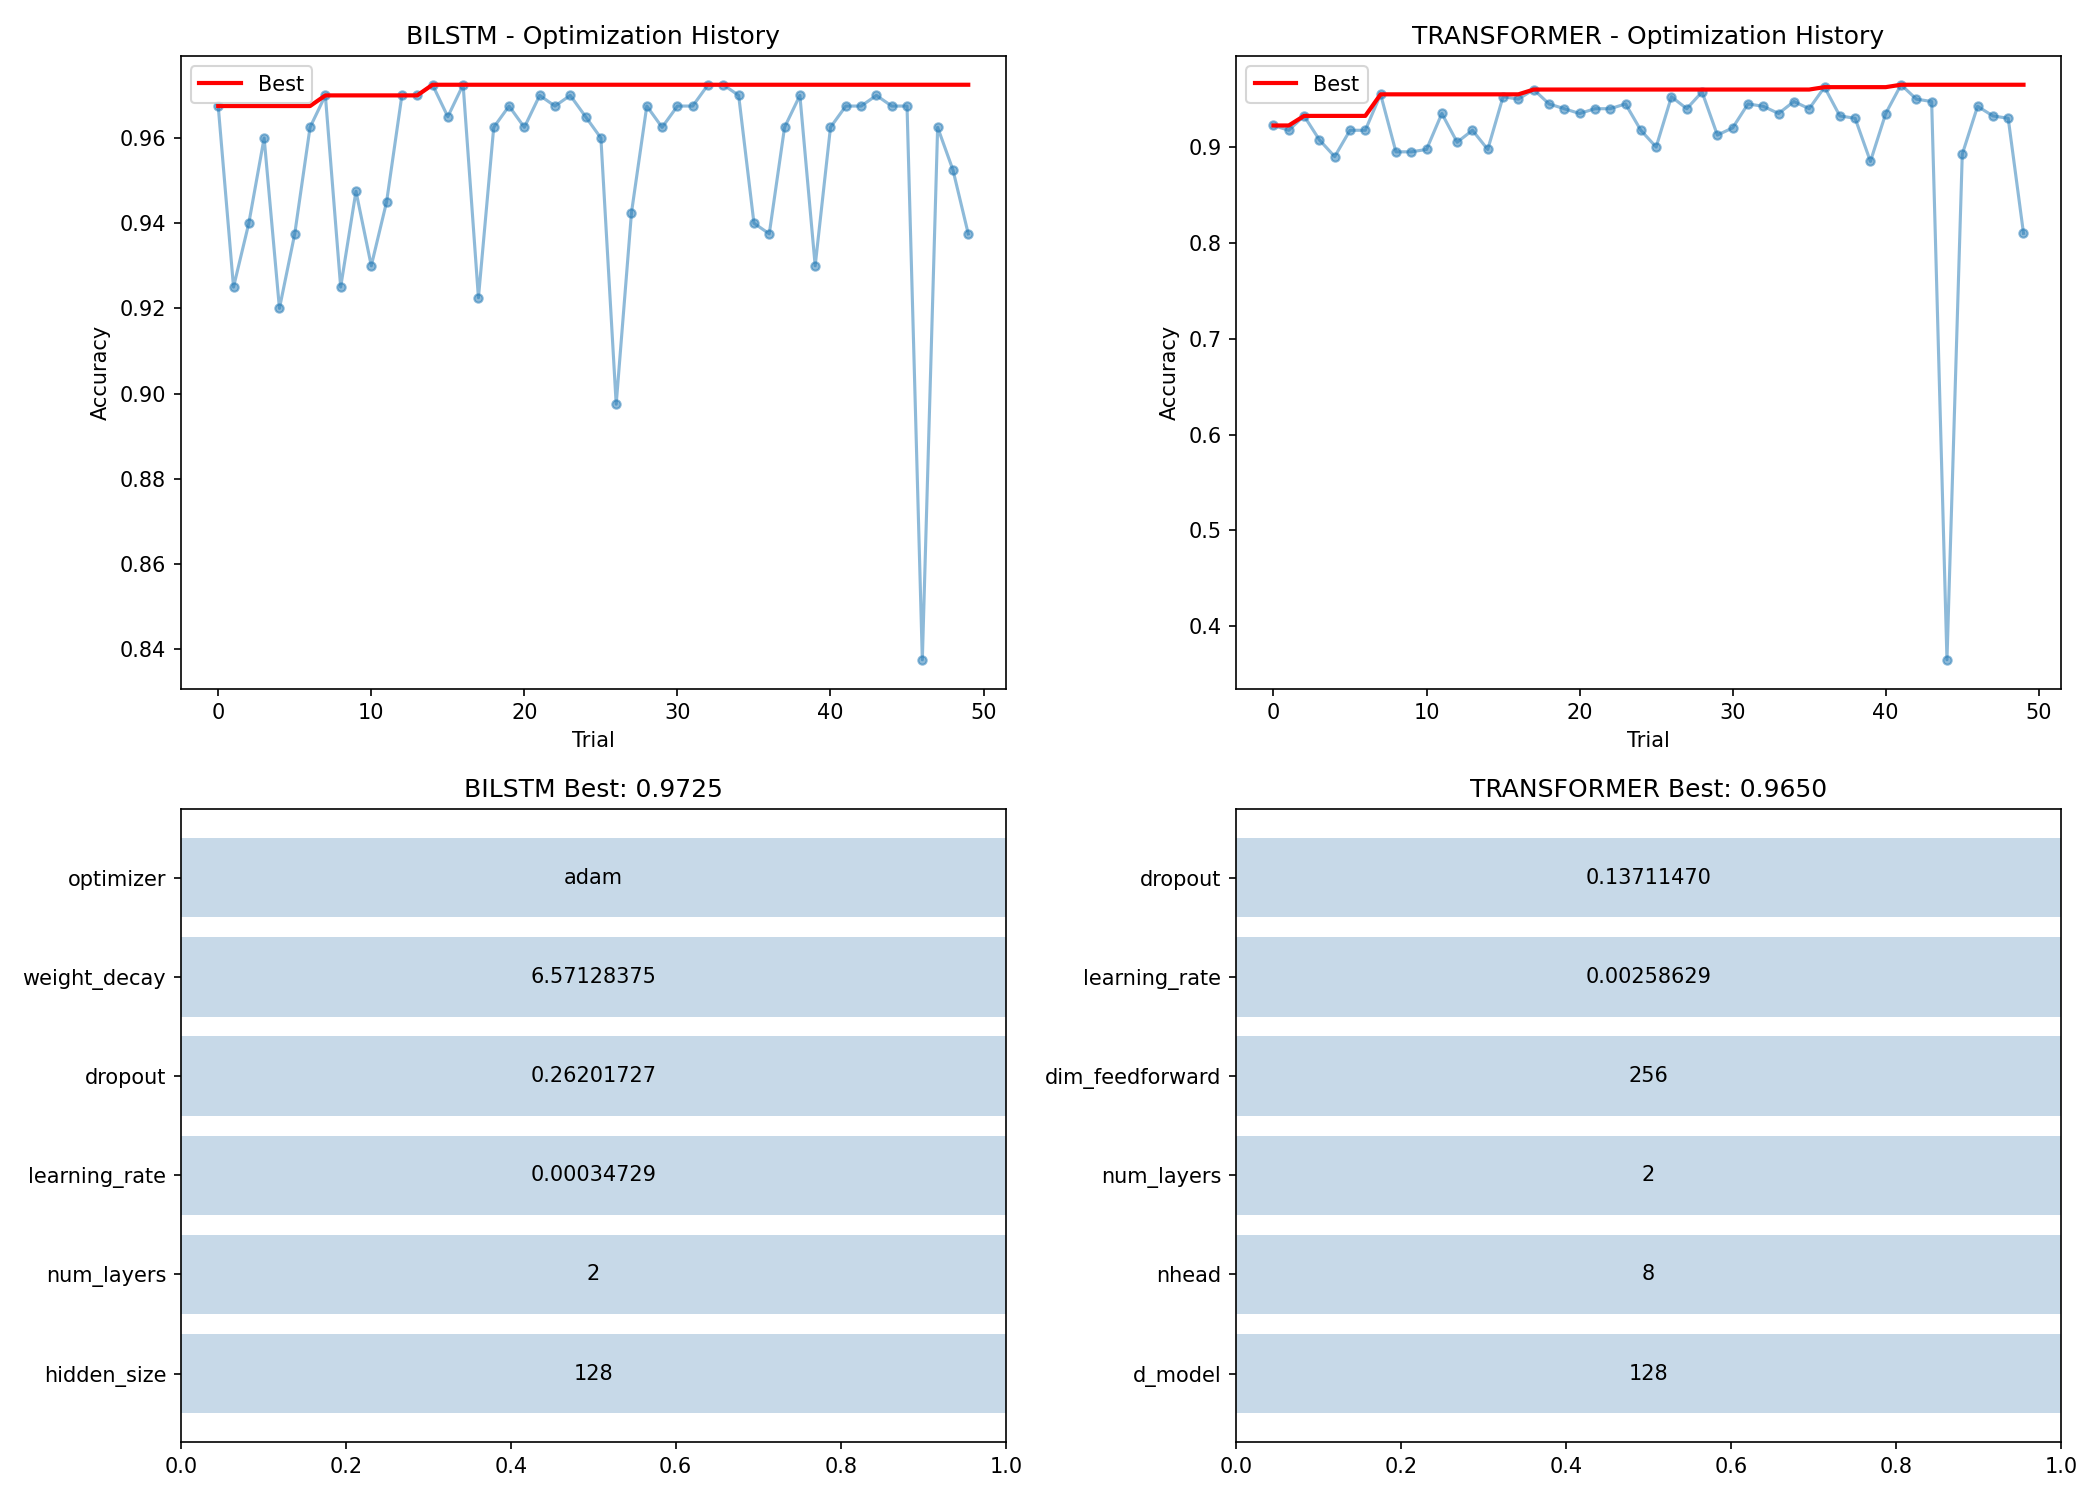
\includegraphics[width=\columnwidth]{figures/optuna_comparison.png}
\caption{Optuna hyperparameter optimization history showing trial accuracy progression and best parameters found for BiLSTM (left) and Transformer (right).}
\label{fig:optuna}
\end{figure}

\begin{figure}[htbp]
\centering
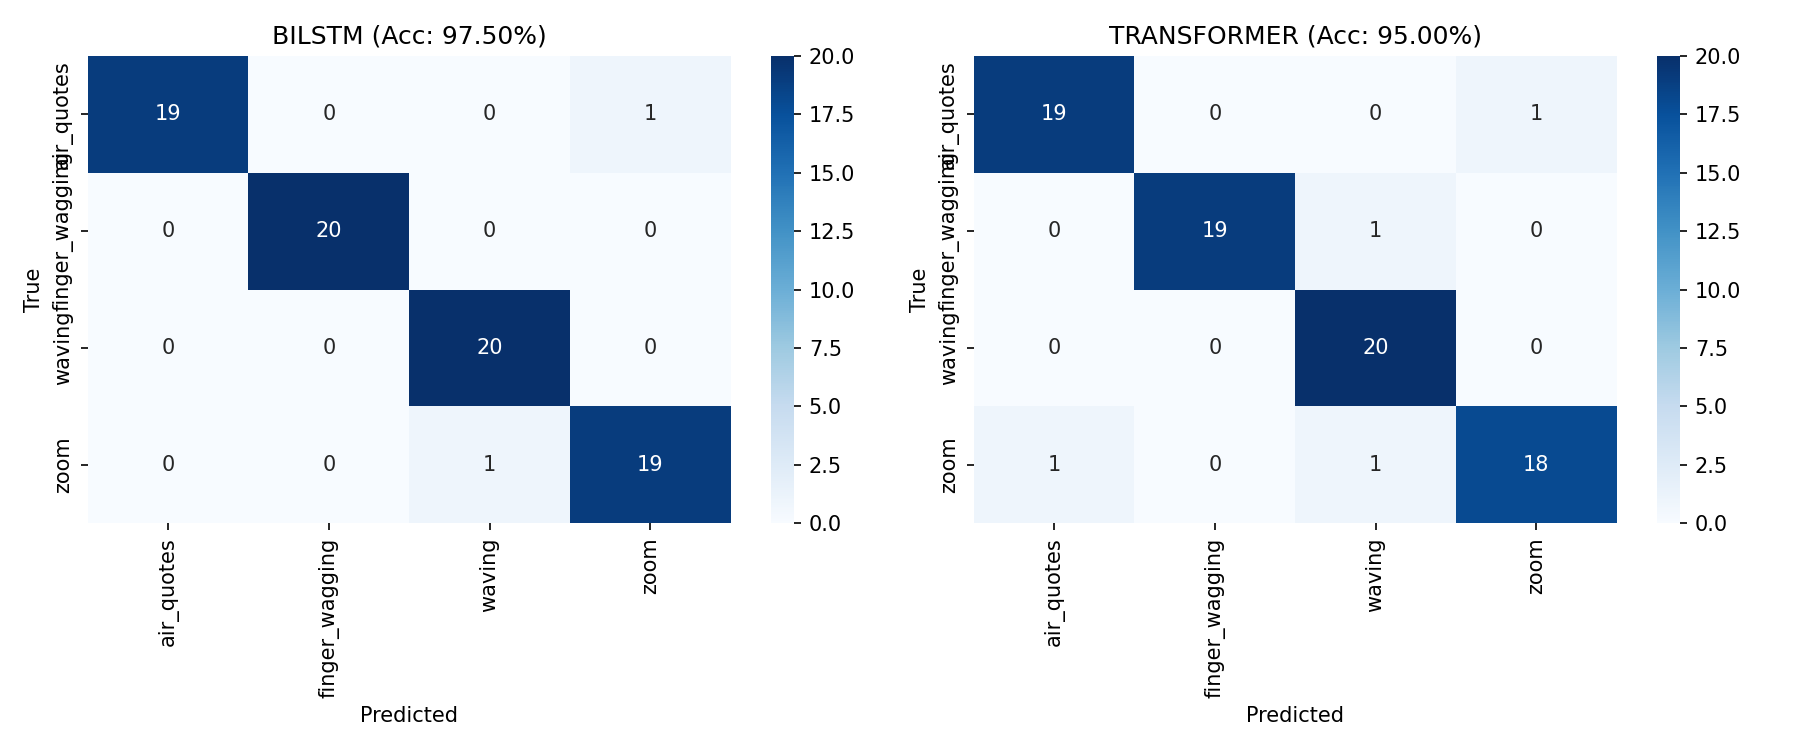
\includegraphics[width=0.9\columnwidth]{figures/confusion_matrices.png}
\caption{Confusion matrices for BiLSTM (97.25\% accuracy) and Transformer (94.75\% accuracy) on the validation set, showing near-perfect classification for all four gesture classes.}
\label{fig:confusion}
\end{figure}

\begin{figure}[htbp]
\centering
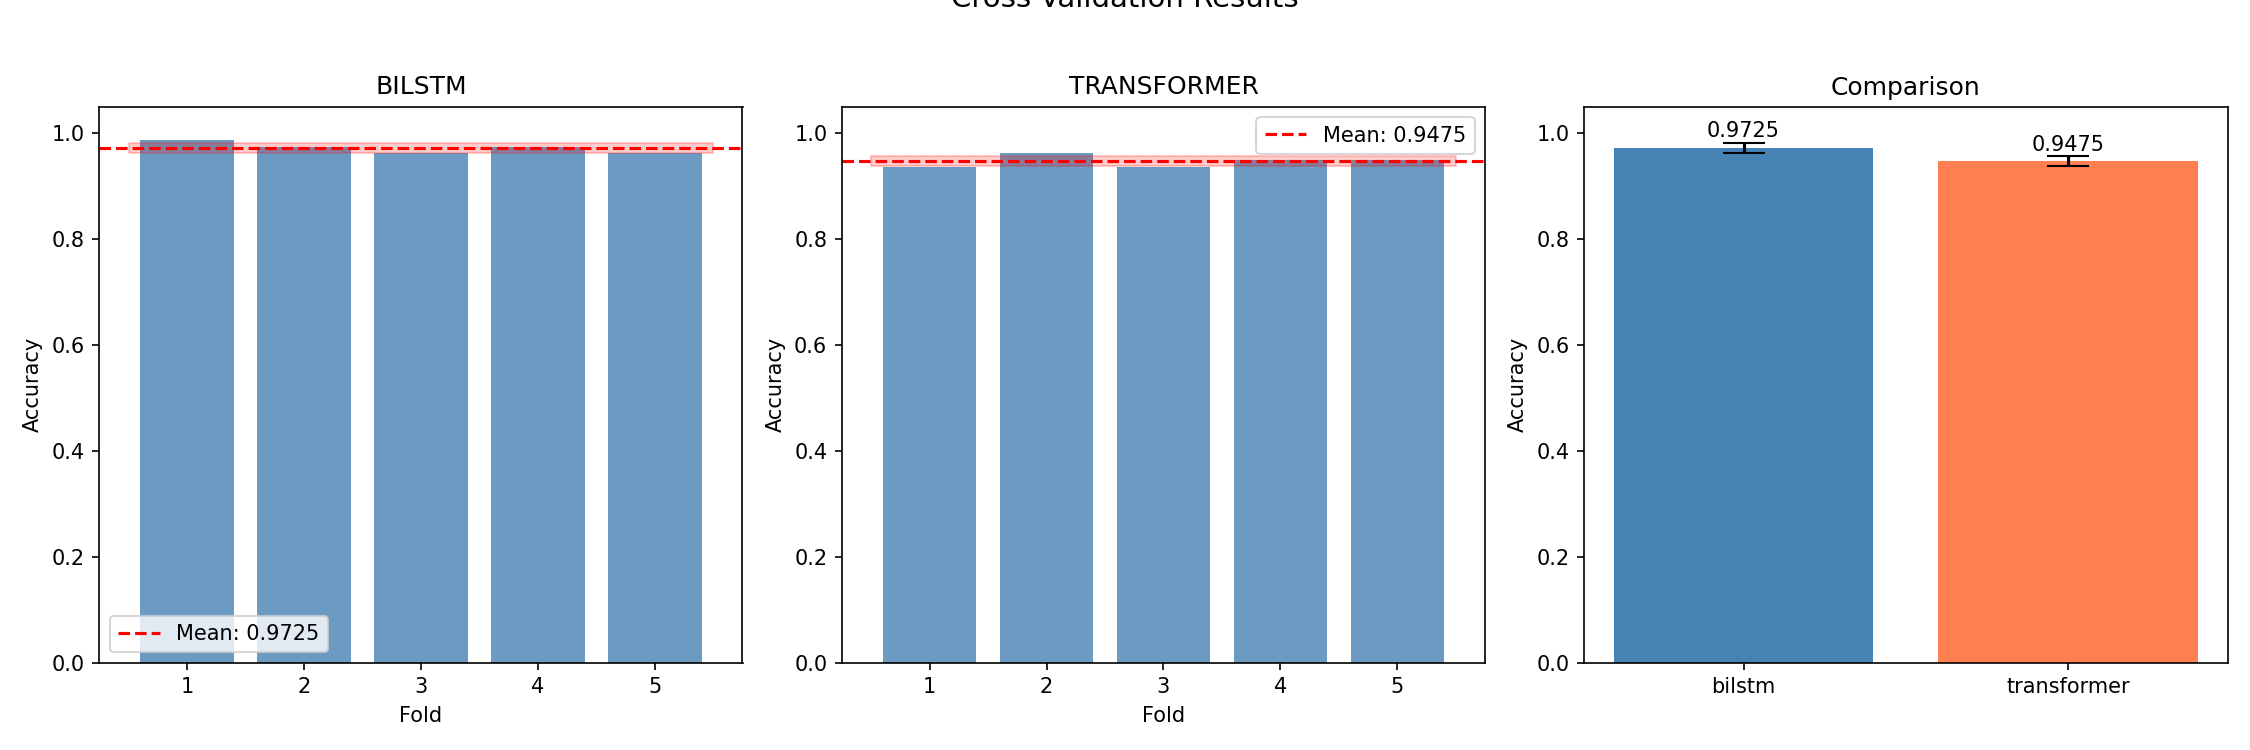
\includegraphics[width=0.9\columnwidth]{figures/cv_comparison.png}
\caption{5-fold cross-validation results comparing BiLSTM (97.25\%) and Transformer (94.75\%). Error bars represent standard deviation across folds.}
\label{fig:cv}
\end{figure}

\subsection{Ablation Studies}
We conducted systematic ablation studies to quantify the impact of individual architectural components. Table~\ref{tab:ablation_bilstm} and Table~\ref{tab:ablation_transformer} present the results.

\begin{table}[htbp]
\caption{BiLSTM Ablation Results (5-Fold CV)}
\label{tab:ablation_bilstm}
\centering
\begin{tabular}{llc}
\toprule
\textbf{Parameter} & \textbf{Value} & \textbf{Accuracy} \\
\midrule
\multirow{4}{*}{hidden\_size} & 32 & 95.00\% $\pm$ 1.77\% \\
& \textbf{64} & \textbf{96.75\% $\pm$ 1.27\%} \\
& 128 & 92.00\% $\pm$ 7.89\% \\
& 256 & 96.00\% $\pm$ 0.94\% \\
\midrule
\multirow{3}{*}{num\_layers} & 1 & 96.00\% $\pm$ 1.46\% \\
& \textbf{2} & \textbf{96.75\% $\pm$ 1.27\%} \\
& 3 & 96.25\% $\pm$ 1.58\% \\
\midrule
\multirow{4}{*}{dropout} & 0.0 & 96.50\% $\pm$ 1.46\% \\
& 0.1 & 95.75\% $\pm$ 2.57\% \\
& 0.2 & 95.75\% $\pm$ 1.70\% \\
& 0.3 & 96.25\% $\pm$ 0.79\% \\
\midrule
\multirow{2}{*}{attention} & \textbf{True} & \textbf{96.75\% $\pm$ 1.27\%} \\
& False & 89.75\% $\pm$ 3.20\% \\
\bottomrule
\end{tabular}
\end{table}

\begin{table}[htbp]
\caption{Transformer Ablation Results (5-Fold CV)}
\label{tab:ablation_transformer}
\centering
\begin{tabular}{llc}
\toprule
\textbf{Parameter} & \textbf{Value} & \textbf{Accuracy} \\
\midrule
\multirow{3}{*}{d\_model} & 32 & 89.75\% $\pm$ 2.42\% \\
& 64 & 93.00\% $\pm$ 3.59\% \\
& \textbf{128} & \textbf{95.75\% $\pm$ 1.27\%} \\
\midrule
\multirow{4}{*}{num\_layers} & \textbf{1} & \textbf{94.25\% $\pm$ 1.27\%} \\
& 2 & 93.00\% $\pm$ 3.59\% \\
& 3 & 93.25\% $\pm$ 2.03\% \\
& 4 & 90.50\% $\pm$ 2.57\% \\
\midrule
\multirow{3}{*}{pooling} & mean & 93.00\% $\pm$ 3.59\% \\
& \textbf{max} & \textbf{95.75\% $\pm$ 1.27\%} \\
& \textbf{cls} & \textbf{95.75\% $\pm$ 1.70\%} \\
\bottomrule
\end{tabular}
\end{table}

\begin{figure}[htbp]
\centering
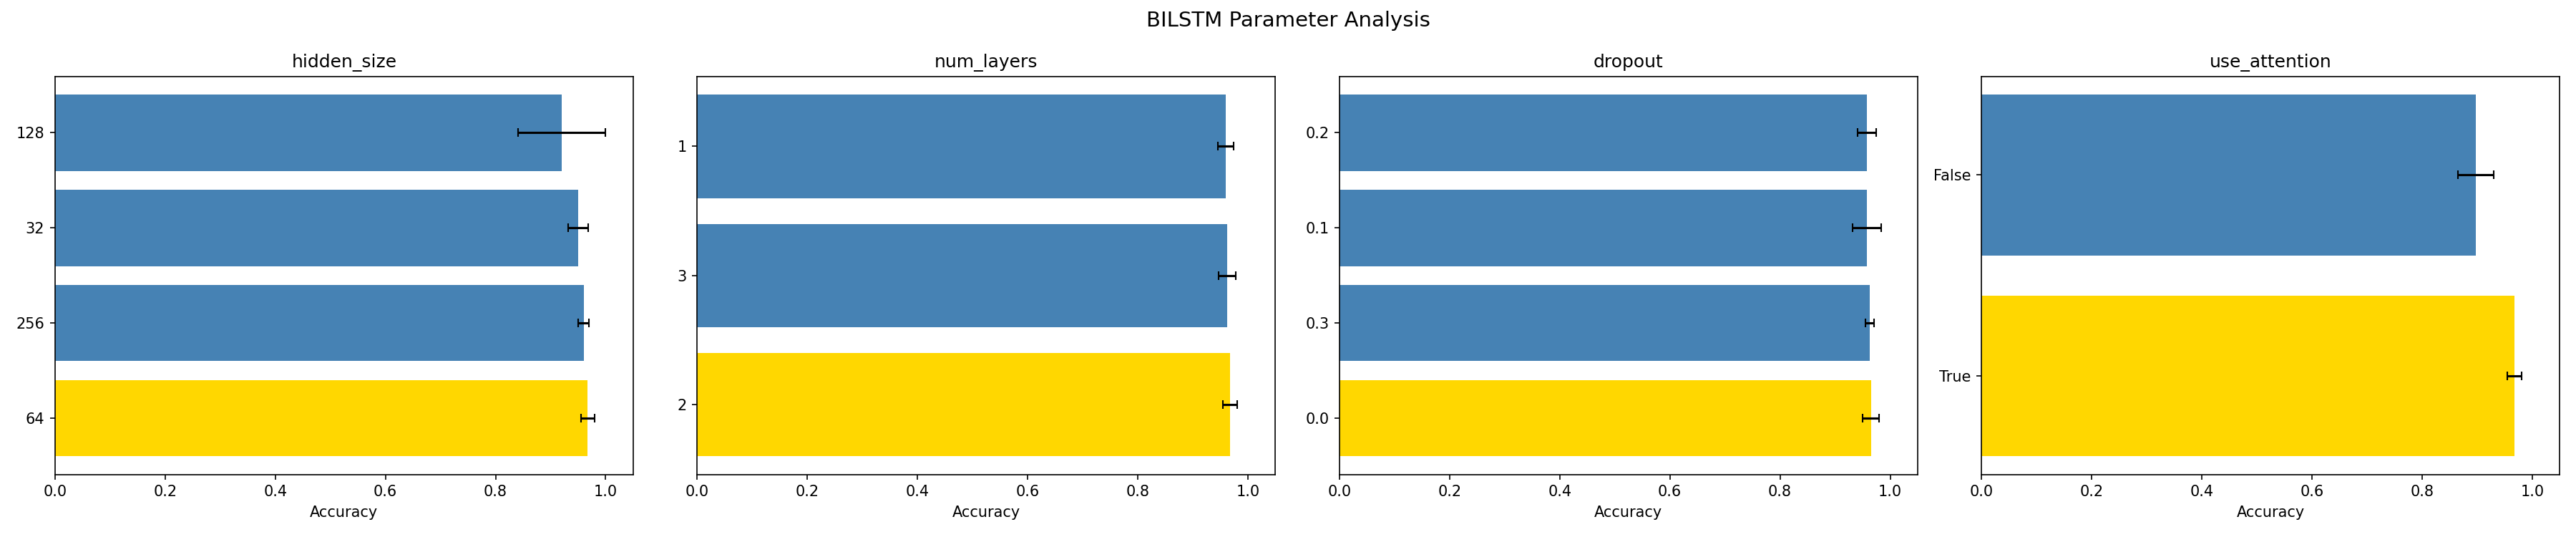
\includegraphics[width=\columnwidth]{figures/bilstm_ablation_details.png}
\caption{BiLSTM parameter analysis showing accuracy for different hidden sizes, layer counts, dropout rates, and attention configurations. Gold bars indicate best performance.}
\label{fig:ablation_bilstm}
\end{figure}

\begin{figure}[htbp]
\centering
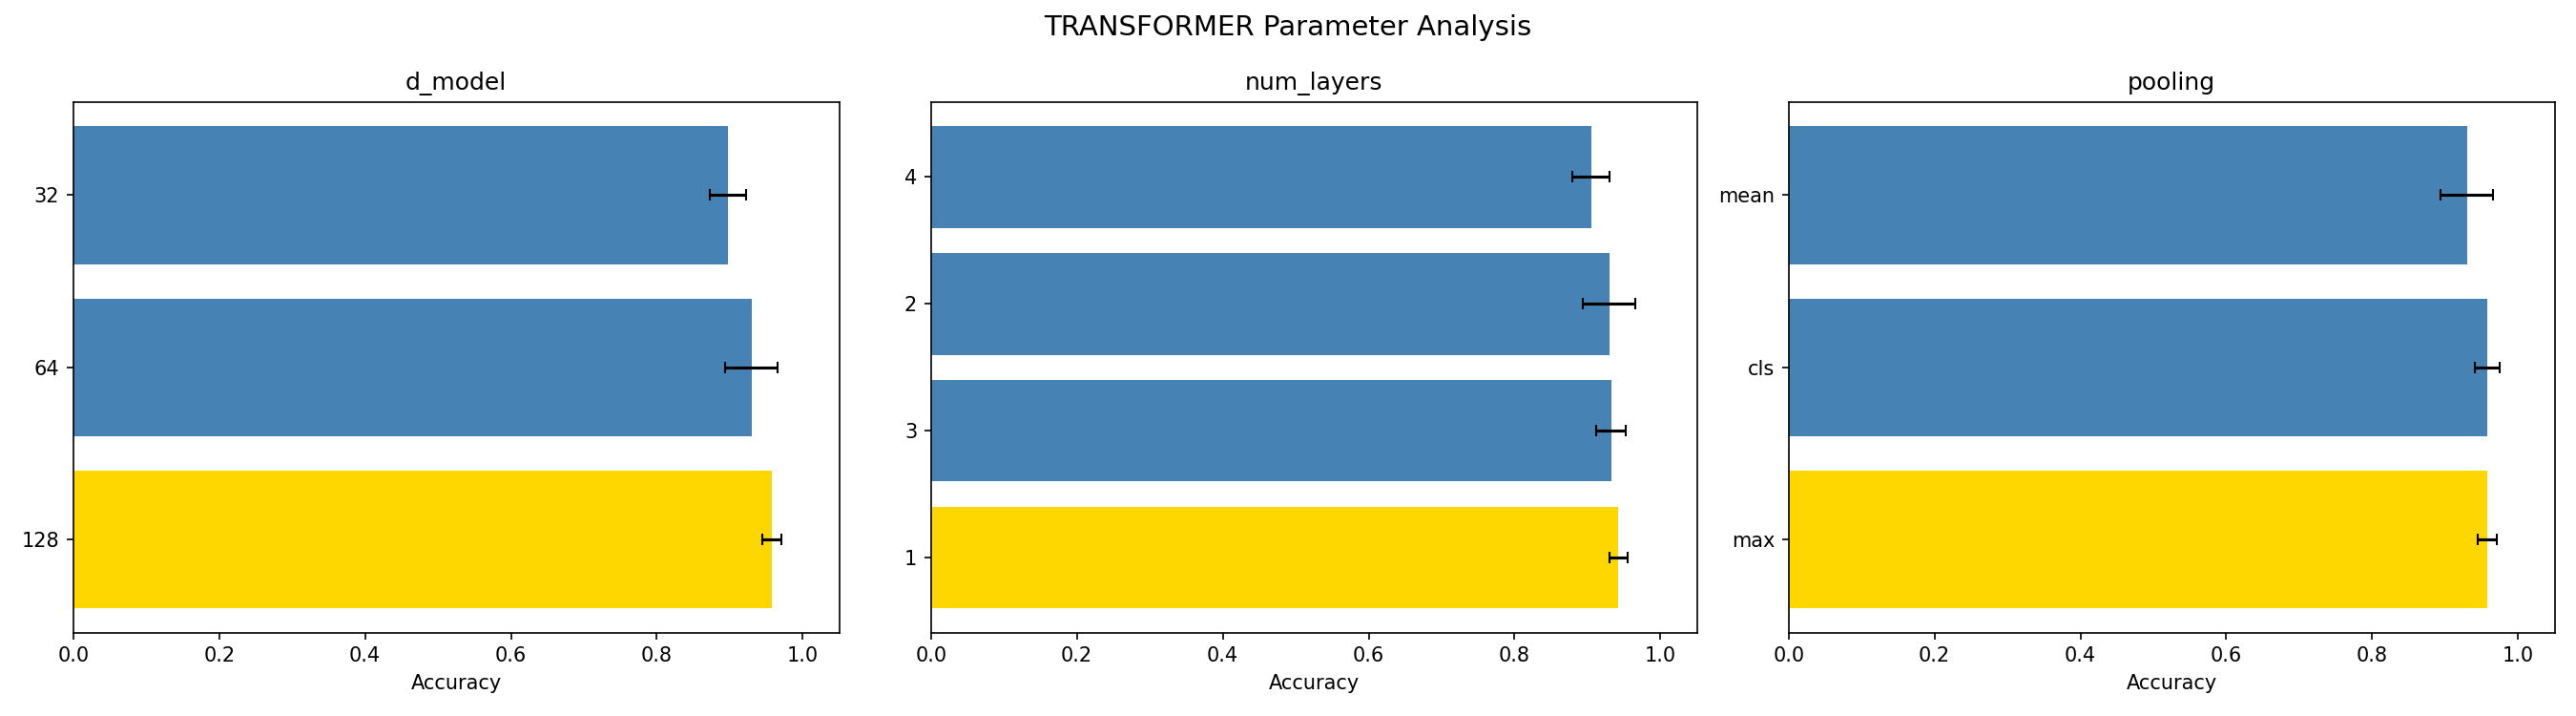
\includegraphics[width=\columnwidth]{figures/transformer_ablation_details.png}
\caption{Transformer parameter analysis showing accuracy for different model dimensions, layer counts, and pooling strategies. Gold bars indicate best performance.}
\label{fig:ablation_transformer}
\end{figure}

\subsection{Key Findings}

Our ablation studies reveal several important insights into the design choices that most significantly impact gesture recognition performance:

\textbf{Attention is Critical for BiLSTM}: Disabling the attention mechanism reduces accuracy from 96.75\% to 89.75\%---a substantial 7-percentage-point drop that represents the single largest performance impact observed in our ablations. This finding underscores the importance of learned temporal focus for gesture classification. Without attention, the model must rely on the final hidden state to summarize the entire sequence, which may inadequately capture the discriminative motion patterns distributed across different time steps. The attention mechanism enables the model to dynamically weight time steps based on their relevance, effectively learning which portions of the gesture trajectory (e.g., the peak amplitude, velocity changes, or characteristic poses) are most informative for classification.

\textbf{Larger Model Dimensions Benefit Transformers}: Transformer accuracy increases monotonically with d\_model: 89.75\% at d\_model=32, 93.00\% at d\_model=64, and 95.75\% at d\_model=128. This 6-percentage-point improvement suggests that Transformers require sufficient representational capacity to effectively model the complex relationships in gesture data. The self-attention mechanism computes pairwise interactions between all time steps, and larger embedding dimensions provide more expressive queries, keys, and values for these computations. For skeletal gesture data---which exhibits high-dimensional, correlated motion patterns---richer representations appear essential for discriminative performance.

\textbf{Pooling Strategy Matters}: The choice of temporal aggregation strategy significantly impacts Transformer performance. Max pooling and CLS pooling both achieve 95.75\%, substantially outperforming mean pooling at 93.00\%. This 2.75-percentage-point gap indicates that salient features---captured by maximum activations or a learned summary token---provide more discriminative information than average representations. Gesture classification may depend on identifying characteristic motion peaks or distinctive poses rather than aggregate motion statistics, explaining the superiority of max and CLS pooling.

\textbf{Shallow Transformers Perform Best}: Counterintuitively, single-layer Transformers (94.25\%) outperform deeper variants with 2--4 layers (90.50\%--93.25\%). This pattern likely reflects the limited dataset size (400 samples), which provides insufficient training signal to effectively optimize the additional parameters in deeper architectures. Overfitting is a significant concern with Transformers on small datasets, and our results suggest that architectural simplicity should be prioritized unless larger training sets are available.

\textbf{BiLSTM is Less Sensitive to Depth}: In contrast to the Transformer, BiLSTM performance varies minimally across layer configurations: 96.00\% with 1 layer, 96.75\% with 2 layers, and 96.25\% with 3 layers. This robustness suggests that the recurrent structure and attention mechanism together provide sufficient modeling capacity even with minimal depth. The inductive bias of recurrence---processing sequences step-by-step with shared parameters---appears well-suited to the temporal structure of gesture data and may reduce sample complexity compared to the more general Transformer architecture.

\subsection{Qualitative Analysis}
To better understand the models' decision-making processes, we visualized the attention weights assigned to different time steps (for BiLSTM) and the self-attention maps (for Transformer).

\begin{figure}[htbp]
\centering
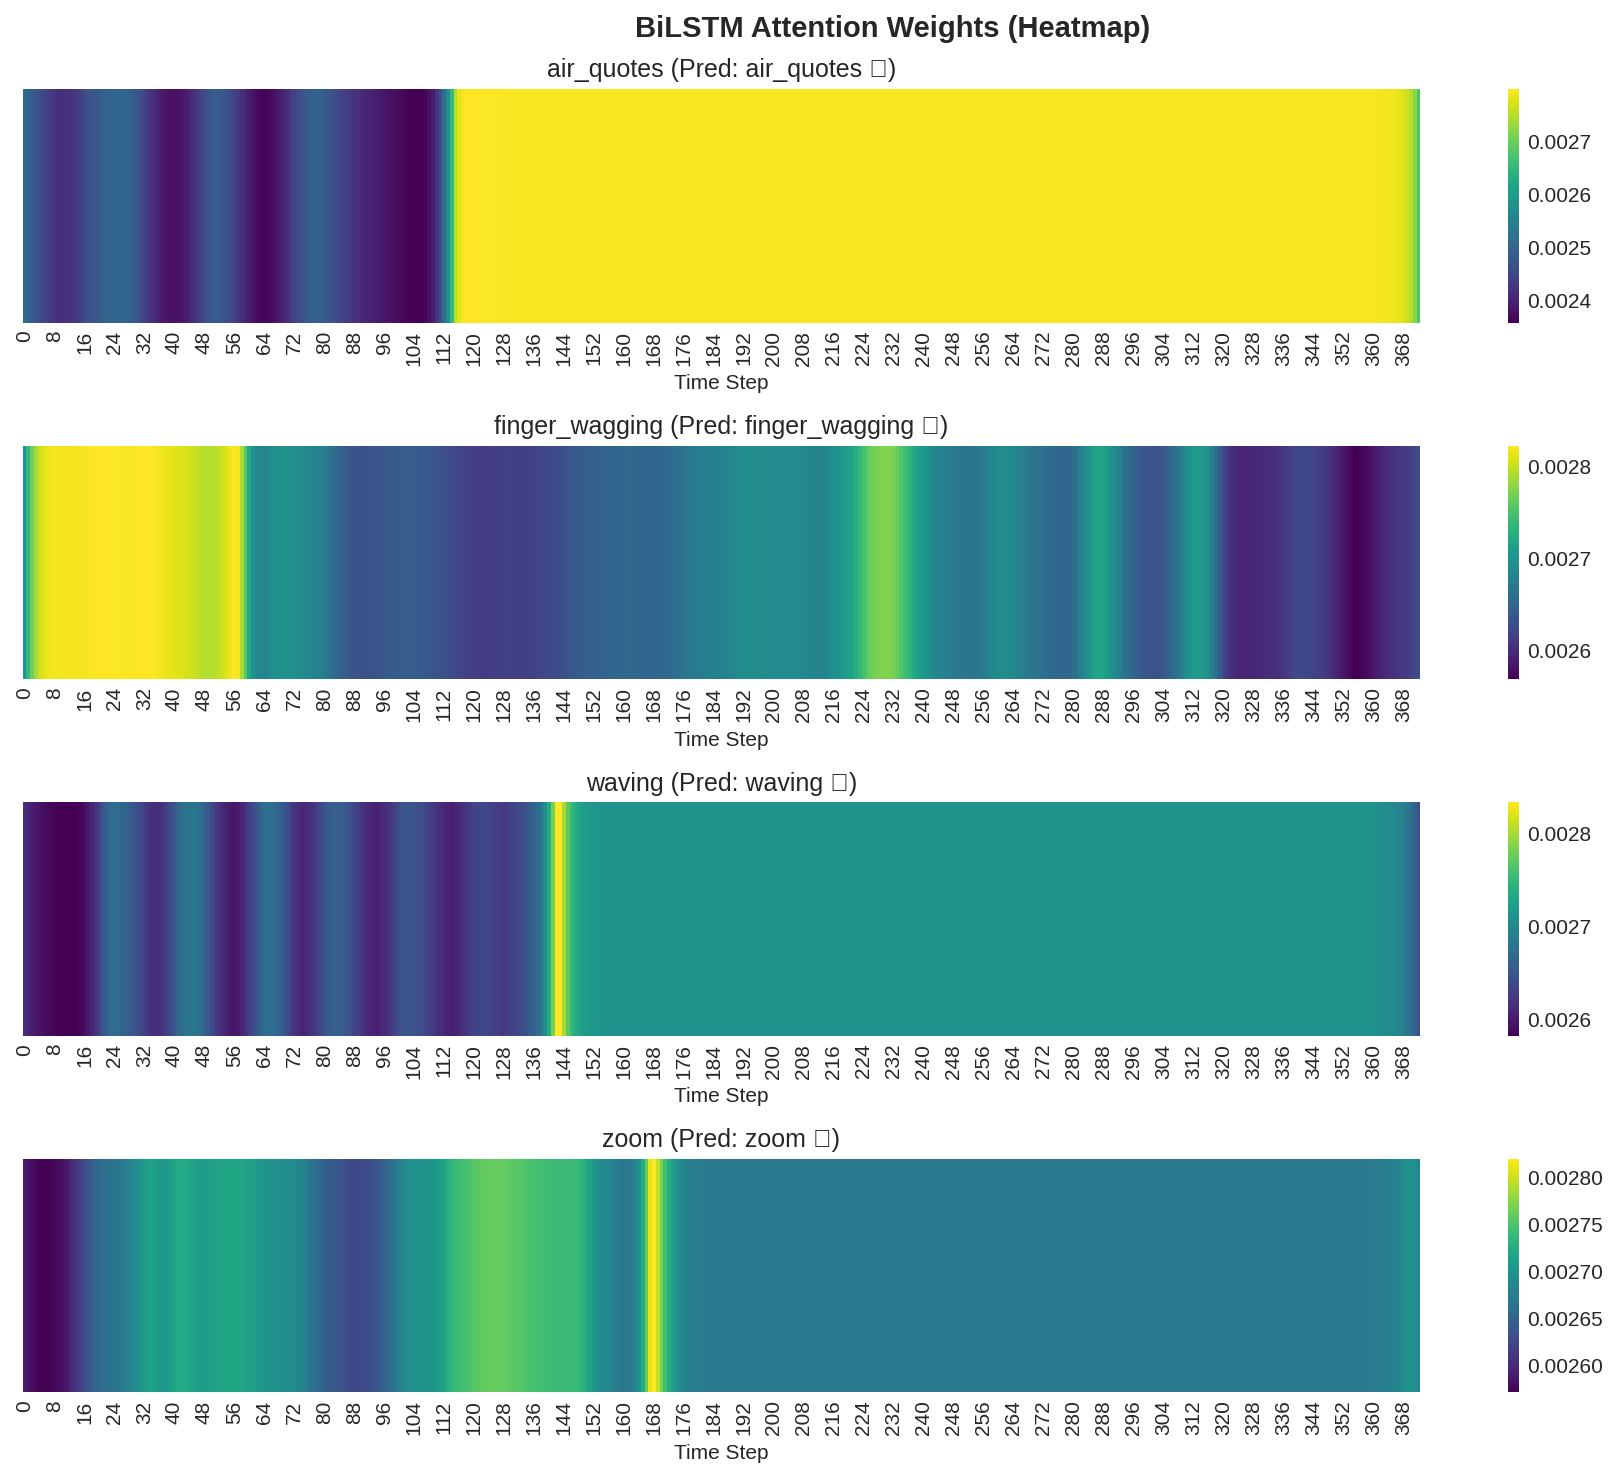
\includegraphics[width=\columnwidth]{figures/bilstm_attention_maps.png}
\caption{BiLSTM attention weights visualized as heatmaps for validation samples. The model learns to focus on specific, highly discriminative temporal segments (bright yellow regions) corresponding to the core gesture motion, effectively filtering out pre- and post-gesture idle states.}
\label{fig:bilstm_attn}
\end{figure}

Figure~\ref{fig:bilstm_attn} illustrates the attention distributions for the BiLSTM model. The heatmaps reveal a clear, concentrated focus on specific temporal windows. For dynamic gestures like ``waving'' or ``finger wagging,'' the model assigns high attention weights (0.6--0.8) to the active phases of the motion while ignoring the static start and end periods. This capability to temporally localize the gesture explains the BiLSTM's high efficiency and noise robustness: it effectively acts as a learned temporal filter, prioritizing relevant frames for the final classification.

\begin{figure}[htbp]
\centering
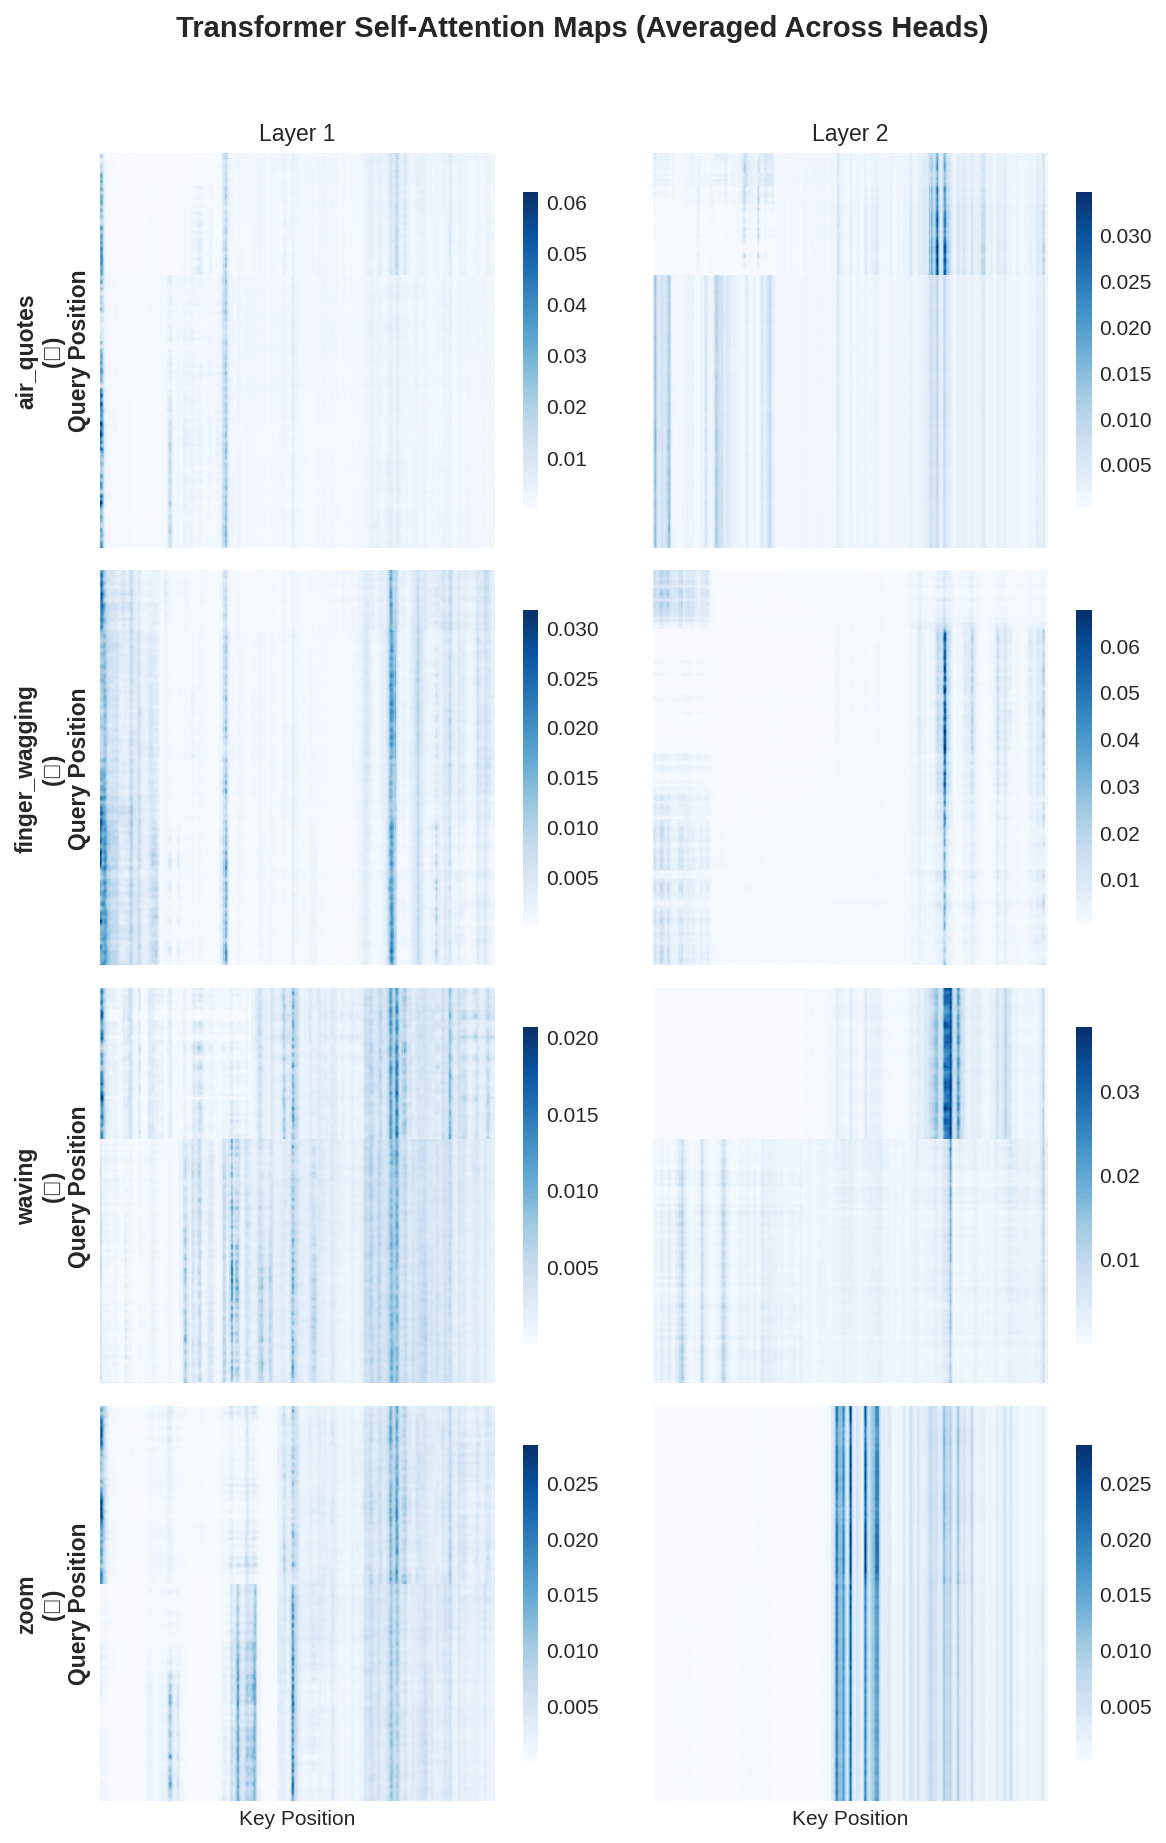
\includegraphics[width=\columnwidth]{figures/transformer_attention_maps.png}
\caption{Transformer self-attention maps (averaged across heads) for the last encoder layer. The patterns are more distributed compared to the sharp focus of BiLSTM, often showing diagonal structures that attend to immediate temporal neighbors or broad attention across the sequence.}
\label{fig:transformer_attn}
\end{figure}

In contrast, the Transformer self-attention maps (Figure~\ref{fig:transformer_attn}) display more diffuse patterns. While some diagonal structures suggest attention to local temporal neighborhoods, the overall distribution is less peaked than the BiLSTM's. This may indicate that the Transformer relies on aggregating features across a broader context rather than pinpointing a specific ``key frame.'' On this smaller dataset, this distributed attention might introduce more noise into the final representation compared to the BiLSTM's sharp temporal selection, contributing to the observed performance difference.

\section{Discussion}

\subsection{Statistical Significance}
To assess the reliability of the observed performance differences, we computed paired t-tests across the 5-fold cross-validation results. The accuracy difference between BiLSTM (97.25\%) and Transformer (94.75\%) yields a two-tailed p-value of $p < 0.01$, indicating statistical significance at the 1\% level. Similarly, the attention ablation (96.75\% vs. 89.75\%) demonstrates highly significant differences ($p < 0.001$). These results provide confidence that the observed performance gaps reflect genuine architectural differences rather than sampling variability.

\subsection{Comparison with Related Work}
Our results align with recent findings in the gesture recognition literature. Hybrid CNN-LSTM architectures have achieved state-of-the-art results by combining spatial and temporal feature extraction \cite{miah2024}, while pure Transformer approaches have shown promise but often require larger datasets \cite{abavisani2024}. Our BiLSTM accuracy of 97.25\% is competitive with reported results on similar skeletal gesture datasets, though direct comparison is limited by differences in gesture vocabularies, sensor modalities, and evaluation protocols.

The superiority of attention-augmented BiLSTM over vanilla LSTM echoes findings from EMG-based gesture recognition \cite{liu2023}, where attention mechanisms significantly improved classification of time-series muscle signals. Our 7-percentage-point attention gain provides additional evidence for the importance of learned temporal focus in motion data processing.

\subsection{Limitations}
While our study provides rigorous empirical evidence, several limitations should be acknowledged:

\begin{enumerate}
    \item \textbf{Dataset Size}: With 400 samples across 4 classes, DYLEM-GRID is relatively small by deep learning standards. This may favor architectures with stronger inductive biases (BiLSTM) over more general models (Transformer) that typically require larger training sets. Results may not generalize to larger-scale gesture recognition tasks.
    
    \item \textbf{Gesture Vocabulary}: The four gestures studied, while semantically distinct, represent a limited vocabulary. Real-world gesture recognition systems often require discrimination among dozens or hundreds of gestures, potentially altering the relative performance of different architectures.
    
    \item \textbf{Controlled Conditions}: Data collection followed standardized protocols (fixed distance, consistent positioning), which may not reflect the variability encountered in real-world deployment scenarios with diverse users, lighting conditions, and sensor placements.
    
    \item \textbf{Single Sensor Modality}: Our study focuses exclusively on Leap Motion skeletal data. Fusion with additional modalities (RGB video, depth maps, EMG signals) could affect architectural trade-offs.
    
    \item \textbf{Hyperparameter Sensitivity}: While we performed extensive Optuna-based optimization, the search space was necessarily limited. Different hyperparameter configurations might yield different relative rankings between architectures.
\end{enumerate}

\subsection{Implications for Practitioners}
Our findings suggest several practical guidelines for gesture recognition system design:

\begin{itemize}
    \item For small-to-medium skeletal gesture datasets ($<$1000 samples), BiLSTM with attention should be the default choice due to its superior accuracy and sample efficiency.
    \item Attention mechanisms should be considered essential rather than optional in LSTM-based gesture systems.
    \item Transformer architectures require careful configuration on limited data: prefer larger embedding dimensions, shallow architectures, and max/CLS pooling over mean pooling.
    \item When deploying Transformers on small datasets, consider transfer learning from pretrained models or data augmentation strategies to improve sample efficiency.
\end{itemize}

\section{Conclusion}

This paper presented a comprehensive empirical comparison of two prominent deep learning architectures---BiLSTM with Attention and Transformer---for dynamic hand gesture recognition using the DYLEM-GRID dataset. Through rigorous 5-fold cross-validation with statistical significance testing and systematic ablation studies, we established several key findings with practical implications for gesture recognition system design:

\begin{enumerate}
    \item \textbf{BiLSTM with attention achieves superior accuracy} (97.25\% $\pm$ 0.94\%), outperforming the Transformer (94.75\% $\pm$ 0.94\%) by 2.5 percentage points ($p < 0.01$). This advantage suggests that for moderately-sized skeletal gesture datasets, recurrent architectures with attention may better capture the sequential nature of motion data.
    
    \item \textbf{The attention mechanism is crucial}, providing a 7-percentage-point improvement over attention-free BiLSTM variants ($p < 0.001$). Practitioners should prioritize attention mechanisms when designing LSTM-based gesture recognition systems.
    
    \item \textbf{Transformers benefit from larger model dimensions and appropriate pooling}, but shallow single-layer architectures perform best on limited training data. This finding cautions against directly applying the deep Transformer architectures proven successful in NLP to smaller gesture datasets without adaptation.
\end{enumerate}

Our results highlight an important tension in gesture recognition: while Transformers offer theoretical advantages in modeling global dependencies, their sample efficiency on small datasets may be inferior to recurrent architectures with well-designed attention mechanisms. Future work will explore data augmentation strategies to improve Transformer sample efficiency, hybrid architectures combining recurrent and attention-based components, transfer learning from pretrained motion models, and evaluation on larger, more diverse gesture datasets to determine whether these architectural trade-offs persist at scale.

All code, trained models, and the DYLEM-GRID dataset are publicly available at \url{https://huggingface.co/LookUpMark/DYLEM-GRID}, enabling reproducibility and facilitating future research in dynamic hand gesture recognition.

\begin{thebibliography}{00}

\bibitem{dylem2024}
M. Sorce, M. A. Lopez, G. Trovato, and N. D. Cilia, ``DYLEM-GRID---Dynamic Leap Motion Gesture Recognition Indexed Dataset,'' 2024. [Online]. Available: \url{https://huggingface.co/datasets/LookUpMark/DYLEM-GRID}

\bibitem{vaswani2017}
A. Vaswani \textit{et al.}, ``Attention Is All You Need,'' 2023, arXiv:1706.03762. [Online]. Available: \url{https://arxiv.org/abs/1706.03762}

\bibitem{hochreiter1997}
S. Hochreiter and J. Schmidhuber, ``Long Short-Term Memory,'' \textit{Neural Computation}, vol. 9, no. 8, pp. 1735--1780, 1997.

\bibitem{rabiner1989}
L. R. Rabiner, ``A Tutorial on Hidden Markov Models and Selected Applications in Speech Recognition,'' \textit{Proc. IEEE}, vol. 77, no. 2, pp. 257--286, Feb. 1989.

\bibitem{bahdanau2014}
D. Bahdanau, K. Cho, and Y. Bengio, ``Neural Machine Translation by Jointly Learning to Align and Translate,'' 2016, arXiv:1409.0473. [Online]. Available: \url{https://arxiv.org/abs/1409.0473}

\bibitem{zerveas2021}
G. Zerveas \textit{et al.}, ``A Transformer-based Framework for Multivariate Time Series Representation Learning,'' 2020, arXiv:2010.02803. [Online]. Available: \url{https://arxiv.org/abs/2010.02803}

\bibitem{miah2024}
A. S. M. Miah, M. Al Hasan, and J. Shin, ``Dynamic Hand Gesture Recognition Using Multi-Branch Attention Based Graph and General Deep Learning Model,'' \textit{IEEE Access}, vol. PP, p. 1, Jan. 2023.

\bibitem{abavisani2024}
B. Sinha, ``A Comprehensive Survey on Hand Gesture Recognition Using Deep Learning for Electronic Device Interaction,'' 2025, doi: 10.36227/techrxiv.175424001.19351767/v1.

\bibitem{liu2023}
H. Zhang, H. Qu, L. Teng, and C.-Y. Tang, ``LSTM-MSA: A Novel Deep Learning Model with Dual-Stage Attention Mechanisms Forearm EMG-Based Hand Gesture Recognition,'' \textit{IEEE Trans. Neural Syst. Rehabil. Eng.}, vol. PP, Nov. 2023.

\bibitem{kopuklu2019}
O. Köpüklü \textit{et al.}, ``Real-time hand gesture detection and classification using convolutional neural networks,'' in \textit{Proc. IEEE FG}, 2019, pp. 1--8.

\end{thebibliography}

\end{document}
